\documentclass{article}
\usepackage[utf8]{inputenc}
\usepackage{polski}
\usepackage{geometry}
\usepackage{pdfpages}
\usepackage{pdfpages}
\usepackage{listings}
\usepackage{listingsutf8}
\usepackage{multirow}
\usepackage{siunitx}
\usepackage{multirow}
\usepackage{booktabs}
\usepackage{tabularx}
\usepackage{placeins}
\usepackage{pdflscape}
\usepackage{colortbl}
\usepackage{listings}
\usepackage{listingsutf8}
\usepackage{pdfpages}
\usepackage[hidelinks]{hyperref}


\geometry{
a4paper,
total={170mm,257mm},
left=20mm,
top=20mm
}
\newcolumntype{Y}{>{\centering\arraybackslash}X}
% \renewcommand\thesection{}
\lstset{%
literate=%
 {ą}{{\k{a}}}1
 {ę}{{\k{e}}}1
 {Ą}{{\k{A}}}1
 {Ę}{{\k{E}}}1
 {ś}{{\'{s}}}1
 {Ś}{{\'{S}}}1
 {ź}{{\'{z}}}1
 {Ź}{{\'{Z}}}1
 {ń}{{\'{n}}}1
 {Ń}{{\'{N}}}1
 {ć}{{\'{c}}}1
 {Ć}{{\'{C}}}1
 {ó}{{\'{o}}}1
 {Ó}{{\'{O}}}1
 {ż}{{\.{z}}}1
 {Ż}{{\.{Z}}}1
 {ł}{{\l{}}}1
 {Ł}{{\l{}}}1
}

\title{Technika Cyfrowa\\
Sprawozdanie - FPGA}
\author{Maciej Trątnowiecki}
\date{AGH, Semestr Letni, 2020}

\begin{document}
\lstset{ 
  backgroundcolor=\color{white},   % choose the background color; you must add \usepackage{color} or \usepackage{xcolor}; should come as last argument
  basicstyle=\footnotesize,        % the size of the fonts that are used for the code
  breakatwhitespace=false,         % sets if automatic breaks should only happen at whitespace
  breaklines=true,                 % sets automatic line breaking
  captionpos=b,                    % sets the caption-position to bottom
  commentstyle=\color{mygreen},    % comment style
  deletekeywords={...},            % if you want to delete keywords from the given language
  escapeinside={\%*}{*)},          % if you want to add LaTeX within your code
  %extendedchars=true,              % lets you use non-ASCII characters; for 8-bits encodings only, does not work with UTF-8
  firstnumber=1000,                % start line enumeration with line 1000
  frame=single,	                   % adds a frame around the code
  keepspaces=true,                 % keeps spaces in text, useful for keeping indentation of code (possibly needs columns=flexible)
  keywordstyle=\color{blue},       % keyword style
  morekeywords={*,...},            % if you want to add more keywords to the set
  numbers=left,                    % where to put the line-numbers; possible values are (none, left, right)
  numbersep=5pt,                   % how far the line-numbers are from the code
  numberstyle=\tiny\color{mygray}, % the style that is used for the line-numbers
  rulecolor=\color{black},         % if not set, the frame-color may be changed on line-breaks within not-black text (e.g. comments (green here))
  showspaces=false,                % show spaces everywhere adding particular underscores; it overrides 'showstringspaces'
  showstringspaces=false,          % underline spaces within strings only
  showtabs=false,                  % show tabs within strings adding particular underscores
  stepnumber=2,                    % the step between two line-numbers. If it's 1, each line will be numbered
  stringstyle=\color{mymauve},     % string literal style
  tabsize=2,	                   % sets default tabsize to 2 spaces
  title=\lstname                   % show the filename of files included with \lstinputlisting; also try caption instead of title
}
    \maketitle
    \section{Opis zrealizowanego projektu}
        W ramach zadania praktycznego przygotowałem implementację algorytmu wyświetlającego na dwóch wyświetlaczach siedmiosegmentowych animację węża. Algorytm zaimplementowałem w dwóch wersjach - w języku SystemVerilog i VHDL dla płytki rozwojowej Altera UP2 wyposażonej w układ FPGA FLEX 10KE EPF10K70RC240-4 dostępnej pod adresem \url{http://eelinux.ee.usm.maine.edu/courses/ele373/upds.pdf}. Wykorzystałem środowisko Quartus II 9.0SP2, w którym przeprowadziłem symulację działania programu. \\
        
        Sekwencję stanów wyjść wyświetlacza odpowiadającą za wyświetlenie zaplanowanej animacji wyznaczyłem na podstawie dokumentacji zestawu edukacyjnego Altera UP2. Strony opisujące rozmieszczenie segmentów wyświetlacza led na płytce, oraz przypisane im piny układu FPGA zostały dołączone na końcu poniższego sprawozdania.
        \begin{center}
            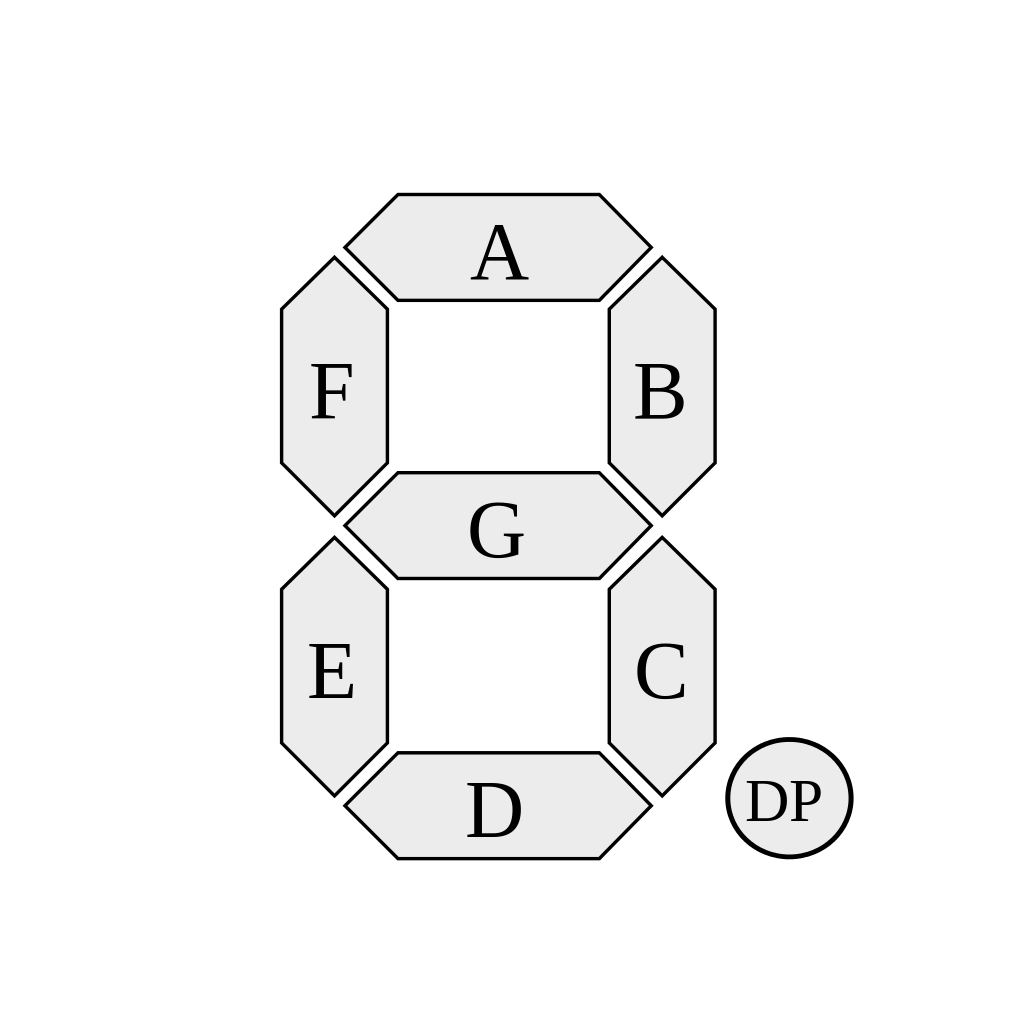
\includegraphics[height=5cm]{reports/img/7seg.png}\\
        \end{center}
        Poniżej zamieszczam przyjętą sekwencję stanów wysokich pozwalających uzyskać zaplanowaną animację.
        \begin{enumerate}
            \item Digit1 G; Digit1 E; Digit1 D
            \item Digit1 E; Digit1 D; Digit2 D
            \item Digit1 D; Digit2 D; Digit2 C
            \item Digit2 D; Digit2 C; Digit2 G
            \item Digit2 C; Digit2 G; Digit1 G
            \item Digit2 G; Digit1 G; Digit1 F
            \item Digit1 G; Digit1 F; Digit1 A
            \item Digit1 F; Digit1 A; Digit2 A
            \item Digit1 A; Digit2 A; Digit2 B
            \item Digit2 A; Digit2 B; Digit2 G
            \item Digit2 B; Digit2 G; Digit1 G
            \item Digit2 G; Digit1 G; Digit1 E
            \item Digit1 G; Digit1 E; Digit1 D
        \end{enumerate}
        Stan opisany numerem 13 jest tożsamy ze stanem początkowym układu. Animacja ma zatem postać dwunastu ustawień wyświetlacza wyświetlanych w cyklu. 
    
    \section{Implementacja w języku SystemVerilog}
        Jako wejście układu przyjęty został sygnał zegarowy (oznaczony clk). Jako wyjście układu zadeklarowano dwie jednowymiarowe macierze typu reg, każda o 7 wyjściach, które następnie zostaną zmapowane do odpowiednich pinów wyświetlacza. Algorytm definiuje też dwie stałe parametryczne znane na etapie kompilacji. Pierwszą z nich jest ITER\_N będącą stałą wewnętrzną układu wskazującą ilość przyjętych stanów animacji. Drugą jest TICKS\_PER\_PHASE określająca co ile taktów zegara nastąpić ma zmiana stanu animacji na kolejny. W programie wykorzystano dwie zmienne lokalne przechowujące liczby naturalne.\\
        
        Ustawione zostało sterowanie zdarzeniowe uruchamiające poniższą logikę za każdym rosnącym zboczem sygnału zegarowego. Jeśli zmienna lokalna odpowiedzialna za zliczanie zaobserwowanych taktów zegara wskazuje na zero, na wyświetlaczu wyświetlona zostaje sekwencja odpowiadająca aktualnemu stanowi symulacji. Następuje inkrementacja zmiennej wskazującej następny stan symulacji. Jeśli zmienna ta wskazuje na wartość równą stałej ITER\_N, zostaje ona wyzerowana. Z każdym taktem procesora następuje inkrementacja zmiennej zliczającej takty. Jeśli zrówna się ona co do wartości ze stałą TICKS\_PER\_PHASE, zostaje wyzerowana.\\
        
        Za wyświetlenie odpowiedniego stanu animacji na wyświetlaczu odpowiedzialne są dwie instrukcje warunkowe \textit{case}. Wartości zmiennych typu reg modyfikowane są poprzez przypisanie odpowiedniej liczby siedmiobitowej zapisanej binarnie.\\
        
        Mechanizm zliczania taktów zegara został zaimplementowany w celu spowolnienia animacji. Jej prędkość zależna jest od częstotliwości sygnału generowanego przez wbudowany w płytkę Altera UP2 układ zegarowy. Zbyt duża prędkość skutkować będzie niskimi walorami estetycznymi. Wielokrotnością spowolnienia sterować można za pomocą stałej parametrycznej TICKS\_PER\_PHASE. Może ona przyjąć wartość dowolnej liczby naturalnej z przedziału $<1,\infty)$.\\
        
        Poniżej zamieszczam kod algorytmu zapisanego w języku SystemVerilog.
        \lstinputlisting[language=Verilog]{../simulations/FPGA/snake_verilog/snake.sv}

        
    \section{Implementacja w języku VHDL}
        Jako wejście układu przyjęty został sygnał zegarowy (oznaczony clk). Jako wyjście układu zadeklarowano dwa wektory wartości logicznych o siedmiu elementach , które następnie zostaną zmapowane do odpowiednich pinów wyświetlacza. Program definiuje też dwie stałe parametryczne znane na etapie kompilacji. Pierwszą z nich jest ITER\_N będącą stałą wewnętrzną układu wskazującą ilość przyjętych stanów animacji. Drugą jest TICKS\_PER\_PHASE określająca co ile taktów zegara nastąpić ma zmiana stanu animacji na kolejny. Może ona przyjmować wartości postaci liczb naturalnych większych lub równych jeden. W programie wykorzystano dwie zmienne lokalne przechowujące liczby naturalne.\\
        
        Program korzysta z biblioteki IEEE, importując moduły odpowiedzialne za standardową logikę i operacje numeryczne. Definiuje także element \textit{snake}, oraz związaną z nim architekturę \textit{arch1}. Wspomniana architektura definiuje procedurę display\_phase przyjmującą jako argument liczbę naturalną. Odpowiedzialna jest ona za wyświetlenie na wyświetlaczu stanu animacji związanego z liczbą przyjętą jako argument. Wykorzystuje do tego instrukcję warunkową \textit{case}, za pomocą której wypełnia wektory odpowiednimi stanami wyjść. Warto zauważyć, że wektory indeksowane są od prawej strony. Stanowi to pewien kontrast do poprzedniego programu, w którym wartości w jednowymiarowej macierzy indeksowane były od lewej strony. Z tego powodu w celu zachowania tej samej kolejności pinów na wyjściu (tzn. kompatybilności z tym samym mapowaniem do pinów wyświetlacza) konieczne jest odbicie lustrzane przypisywanych w wektorach wartości. \\
        
        
        W architekturze \textit{arch1} zarejestrowany jest proces \textit{tick} uruchamiany sygnałem \textit{clk}. Z każdym rosnącym zboczem 
        sygnału zegarowego, przeprowadzana jest analiza logiczna analogiczna do tej zapisanej w języku SystemVerilog. Jeśli licznik taktów wskazuje zero, następuje zmiana stanu animacji za pomocą wcześniej zdefiniowanej procedury, oraz inkrementacja zmiennej identyfikującej następny stan animacji. Jest ona zerowana, gdy zrówna się co do wartości ze stałą ITER\_N. Z każdym taktem zegara następuje inkrementacja licznika taktów, który jest zerowany gdy zrówna się co do wartości ze stałą TICKS\_PER\_PHASE. \\
        
        Algorytm implementuje opóźnienie animacji względem zegara w sposób analogiczny do opisanego w poprzednim punkcie.\\ 
    
        Poniżej zamieszczam kod algorytmu zapisanego w języku VHDL. 
        \lstinputlisting[language=VHDL]{../simulations/FPGA/snake_vhdl/snake.vhd}
    
    \section{Symulacja działania programu}
        Długość symulacji ustaliłem na cztery sekundy. Symulacje oparłem o plik określający kształt fali. Z dokumentacji płytki rozwojowej Altera UP2 odczytać możemy częstotliwość sygnału generowanego przez zegar jako $25.175Mhz$. Oznacza, to że zegar generuje sygnał o okresie $39.7ns$ (jako że okres jest odwrotnością częstotliwości). Jeśli chcielibyśmy otrzymać animację z dziesięcioma zmianami stanu na sekundę, odpowiadałoby to ustawieniu stałej TICKS\_PER\_PHASE na wartość 2717500. W praktyce symulacja o takiej dokładności wymaga sporej mocy obliczeniowej, dlatego na jej potrzeby ustawiłem stałą na 10. Do pliku symulacji dodałem sygnał wejściowy układu zegara o okresie 10 ms. Takie uproszczenie symulacji nie ma wpływu na możliwość pokazania poprawności działania algorytmu. 
        \begin{center}
            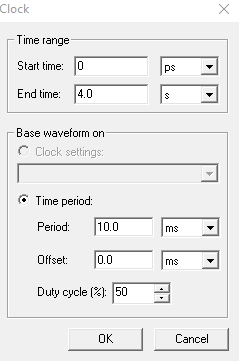
\includegraphics[height=10cm]{reports/img/fpga_clock.png}\\
        \end{center}
        \FloatBarrier
        
        
    
    \section{Przydział pinów}
        W środowisku Quartus II wybrałem układ FLEX 10KE EPF10K70RC240-4 jako urządzenie docelowe dla napisanego programu. Następnie korzystając z funkcji \textit{Pin Planner}, oraz dokumentacji płytki Altera UP2 przygotowałem mapowanie portów algorytmu na odpowiednie piny układu. Pin zegarowy odczytałem z dokumentacji układu EPF10K70RC240-4 dostępnej pod adresem \url{https://www.intel.com/content/dam/www/programmable/us/en/pdfs/literature/dp/flex10k/archives/epf10k70.pdf}. Otrzymałem poniższy układ. 
        
        \begin{center}
            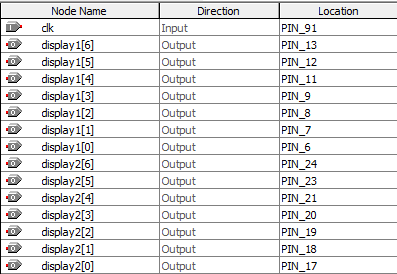
\includegraphics[height=10cm]{reports/img/fpga_1.png}\\
        \end{center}
        
        Tak przygotowane mapowanie pinów układu pozwoli wyświetlić animację na wyświetlaczu dwóch cyfr FLEX\_DIGIT znajdującym się w prawym górnym rogu płytki rozwojowej. 

    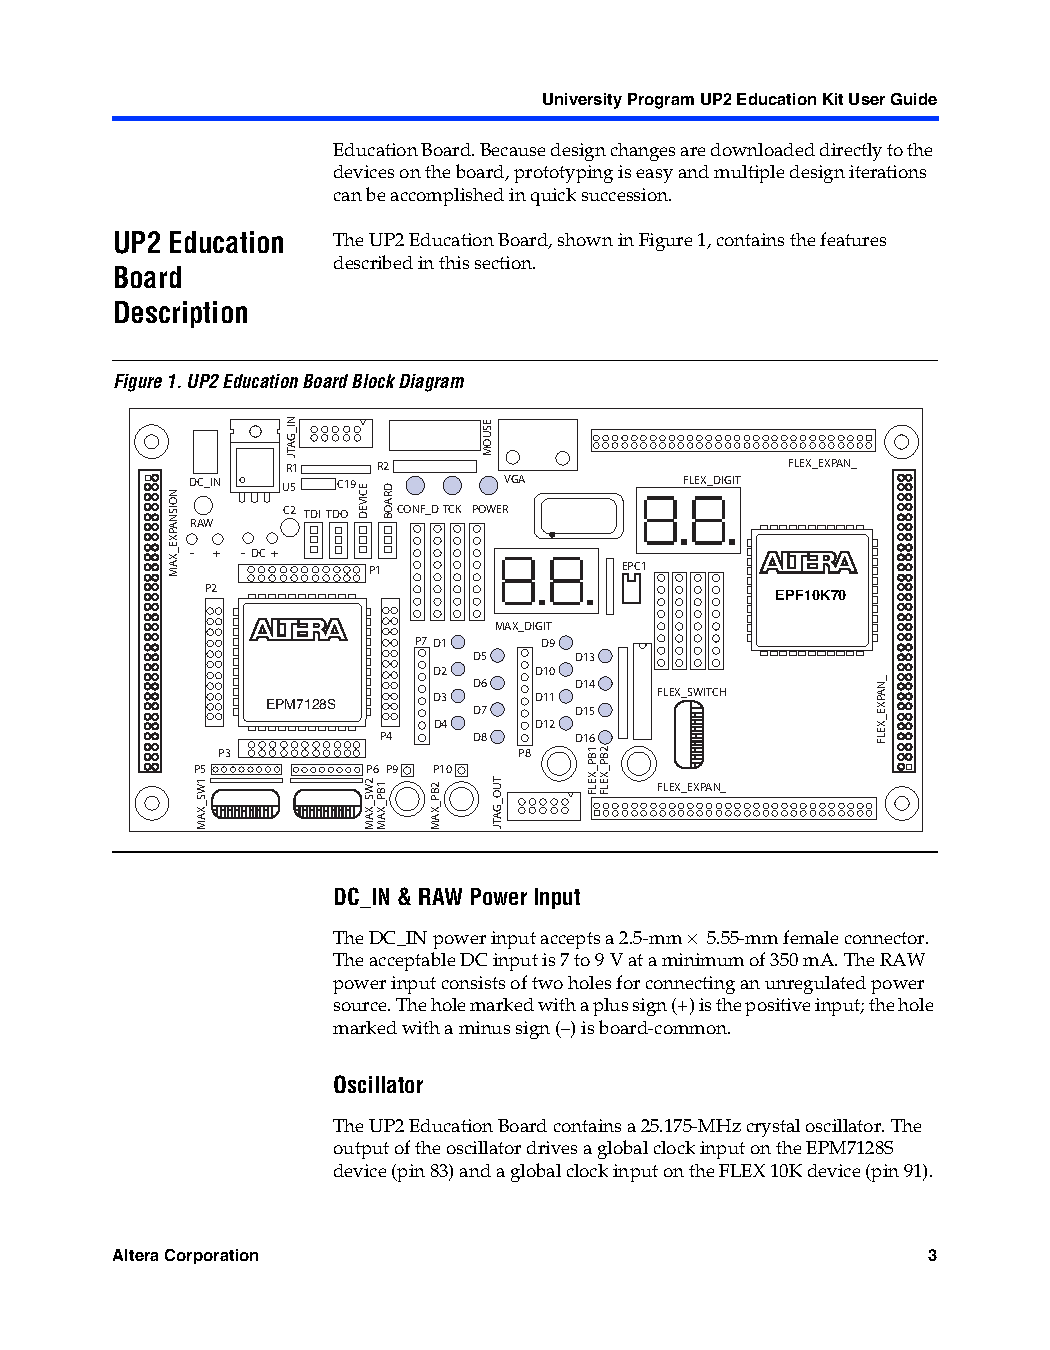
\includepdf{img/docs_p3.pdf}  
    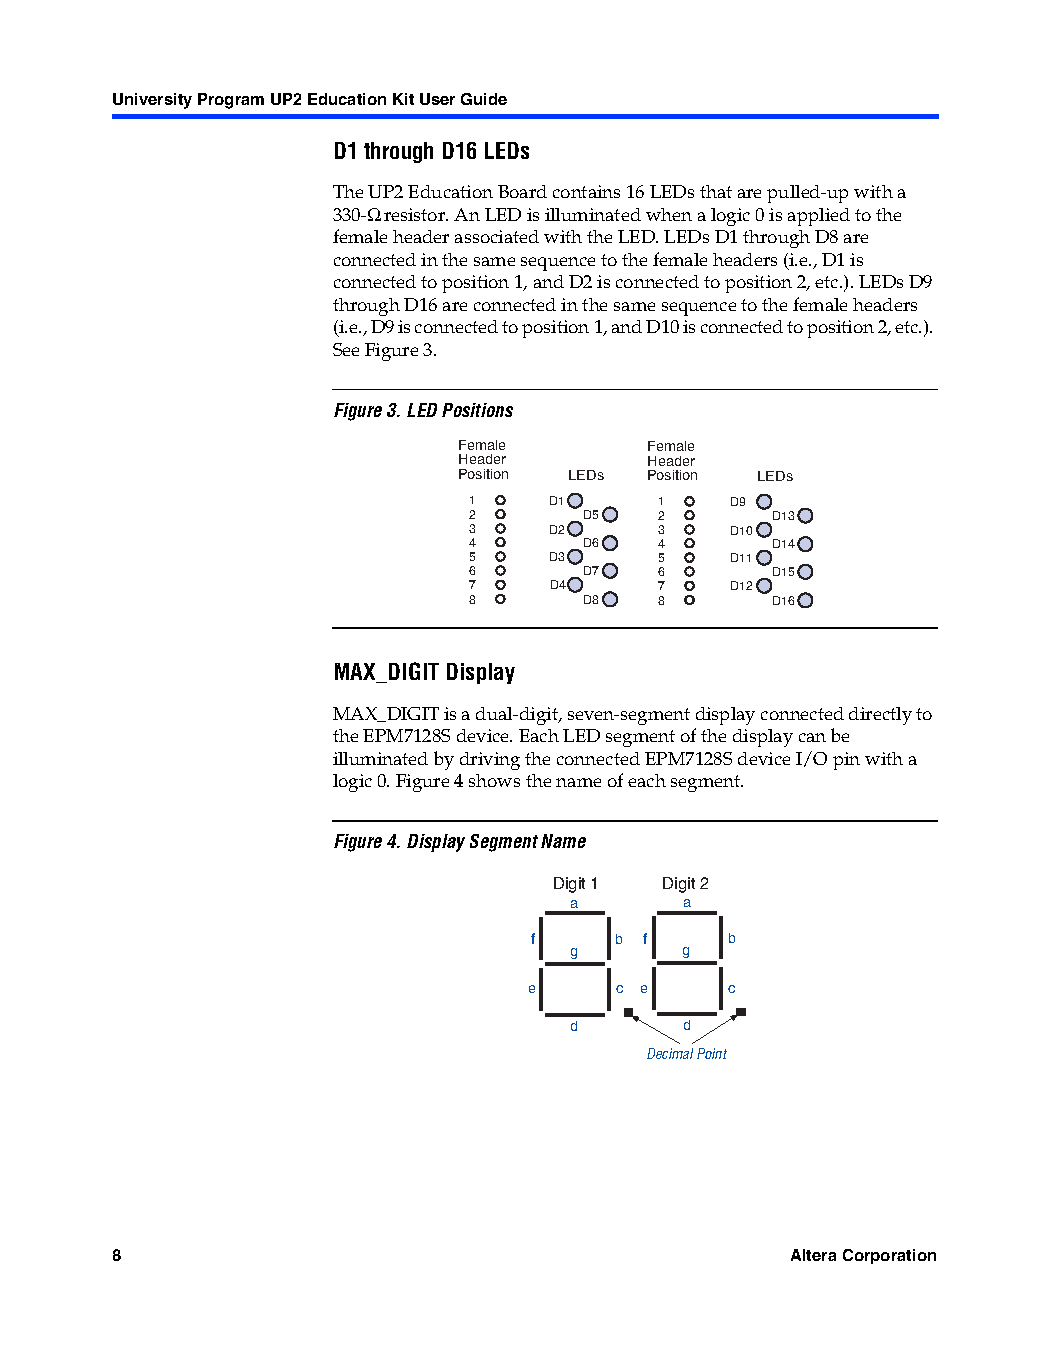
\includepdf{img/docs_p8.pdf}  
    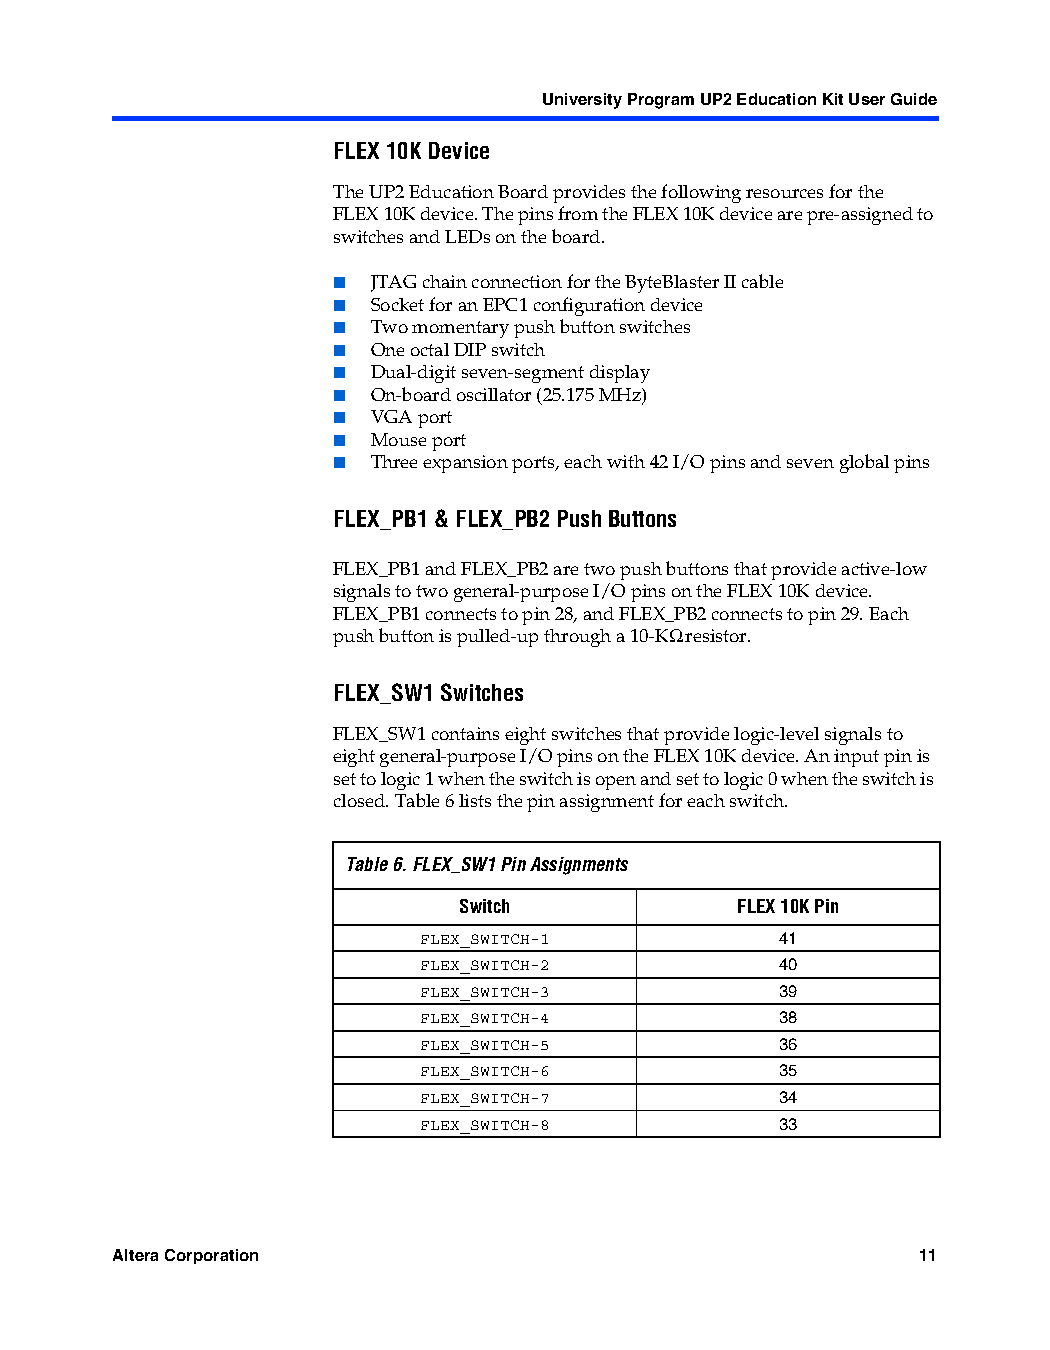
\includepdf{img/docs_p11.pdf}  
    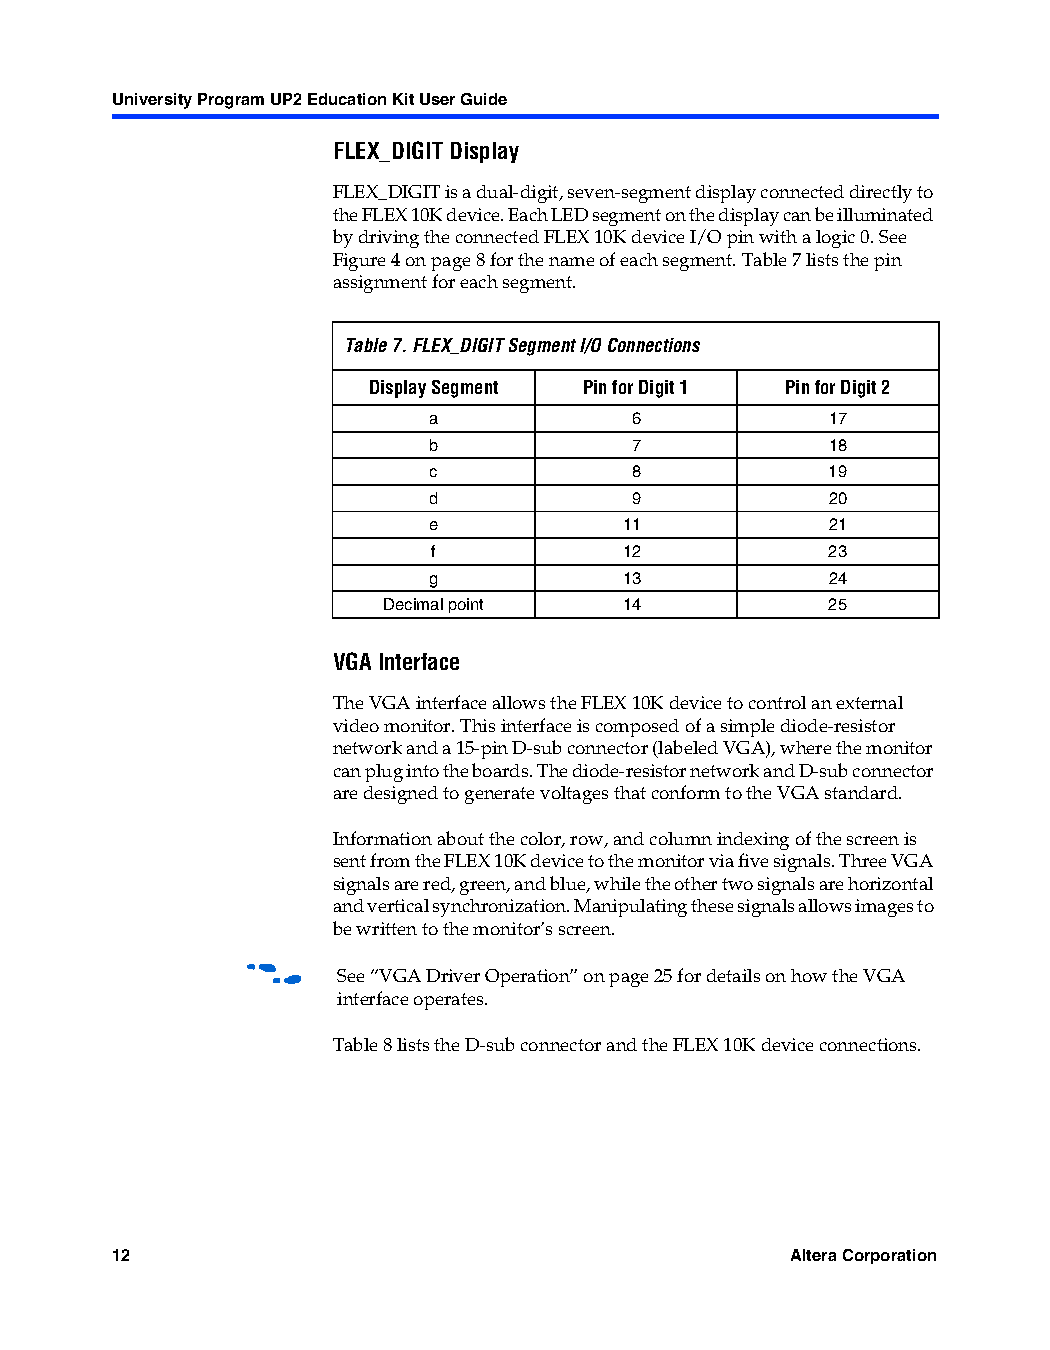
\includepdf{img/docs_p12.pdf}
    
\end{document}
